%%%%%%%%%%%%%%%%%%%%%%%%% 
% Dokumentinformationen %
%%%%%%%%%%%%%%%%%%%%%%%%%
\newcommand{\titleinfo}{Signale und Systeme 1 - Zusammenfassung}
\newcommand{\authorinfo}{Braun \& Co, J.Rast}
\newcommand{\versioninfo}{$Revision: 1 $ - powered by \LaTeX} 

%%%%%%%%%%%%%%%%%%%%%%%%%%%%%%%%%%%%%%%%%%%%%
% Standard projektübergreifender Header für
% - Makros 
% - Farben
% - Mathematische Operatoren
%
% DORT NUR ERGÄNZEN, NICHTS LÖSCHEN
%%%%%%%%%%%%%%%%%%%%%%%%%%%%%%%%%%%%%%%%%%%%%
% Genereller Header
\documentclass[10pt,twoside,a4paper,fleqn]{article}
\usepackage[utf8]{inputenc}
\usepackage[left=1cm,right=1cm,top=1cm,bottom=1cm,includeheadfoot]{geometry}
\usepackage[ngerman]{babel,varioref}

% Pakete
\usepackage{amssymb,amsmath,fancybox,graphicx,color,lastpage,wrapfig,fancyhdr,hyperref,verbatim,multicol}

%%%%%%%%%%%%%%%%%%%%
% Generelle Makros %
%%%%%%%%%%%%%%%%%%%%
\newcommand{\skript}[1]{$_{\textcolor{red}{\mbox{\small{Skript S.#1}}}}$}
\newcommand{\verweis}[2]{\small{(siehe auch \ref{#1}, #2 (S. \pageref{#1}))}}
\newcommand{\subsubadd}[1]{\textcolor{black}{\mbox{#1}}}

\newcommand{\matlab}[1]{\footnotesize{(Matlab: \texttt{#1})}\normalsize{}}

%%%%%%%%%%
% Farben %
%%%%%%%%%%
\definecolor{black}{rgb}{0,0,0}
\definecolor{red}{rgb}{1,0,0}
\definecolor{white}{rgb}{1,1,1}
\definecolor{grey}{rgb}{0.8,0.8,0.8}

%%%%%%%%%%%%%%%%%%%%%%%%%%%%
% Mathematische Operatoren %
%%%%%%%%%%%%%%%%%%%%%%%%%%%%
\DeclareMathOperator{\sinc}{sinc}
\DeclareMathOperator{\sgn}{sgn}
\DeclareMathOperator{\Real}{Re}
\DeclareMathOperator{\Imag}{Im}



% Fouriertransformation
\unitlength1cm
\newcommand{\FT}
{
\begin{picture}(1,0.5)
\put(0.2,0.1){\circle{0.14}}\put(0.27,0.1){\line(1,0){0.5}}\put(0.77,0.1){\circle*{0.14}}
\end{picture}
}

% Inverse Fouriertransformation
\newcommand{\IFT}
{
\begin{picture}(1,0.5)
\put(0.2,0.1){\circle*{0.14}}\put(0.27,0.1){\line(1,0){0.45}}\put(0.77,0.1){\circle{0.14}}
\end{picture}
}



%%%%%%%%%%%%%%%%%%%%%%%%%%%%
% Allgemeine Einstellungen %
%%%%%%%%%%%%%%%%%%%%%%%%%%%%
%PDF Info
\hypersetup{pdfauthor={\authorinfo},pdftitle={\titleinfo},colorlinks=false}
\author{\authorinfo}
\title{\titleinfo}

%Kopf- und Fusszeile
\pagestyle{fancy}
\fancyhf{}
%Linien oben und unten
\renewcommand{\headrulewidth}{0.5pt} 
\renewcommand{\footrulewidth}{0.5pt}

\fancyhead[L]{\titleinfo{ }\tiny{(\versioninfo)}}
%Kopfzeile rechts bzw. aussen
\fancyhead[R]{Seite \thepage { }von \pageref{LastPage}}
%Fusszeile links bzw. innen
\fancyfoot[L]{\footnotesize{\authorinfo}}
%Fusszeile rechts bzw. ausen
\fancyfoot[R]{\footnotesize{\today}}

% Einrücken verhindern versuchen
\setlength{\parindent}{0pt}

% Zeilenhöhe Tabellen:
\renewcommand{\arraystretch}{1.5}



% Möglichst keine Ergänzungen hier, sondern in header.tex
\begin{document}
\section{Signalbeschreibung \skript{1}}
\subsection{Energie- und Leistungssignale \skript{3}}
\begin{tabular}{ll}
\parbox{12cm}{
	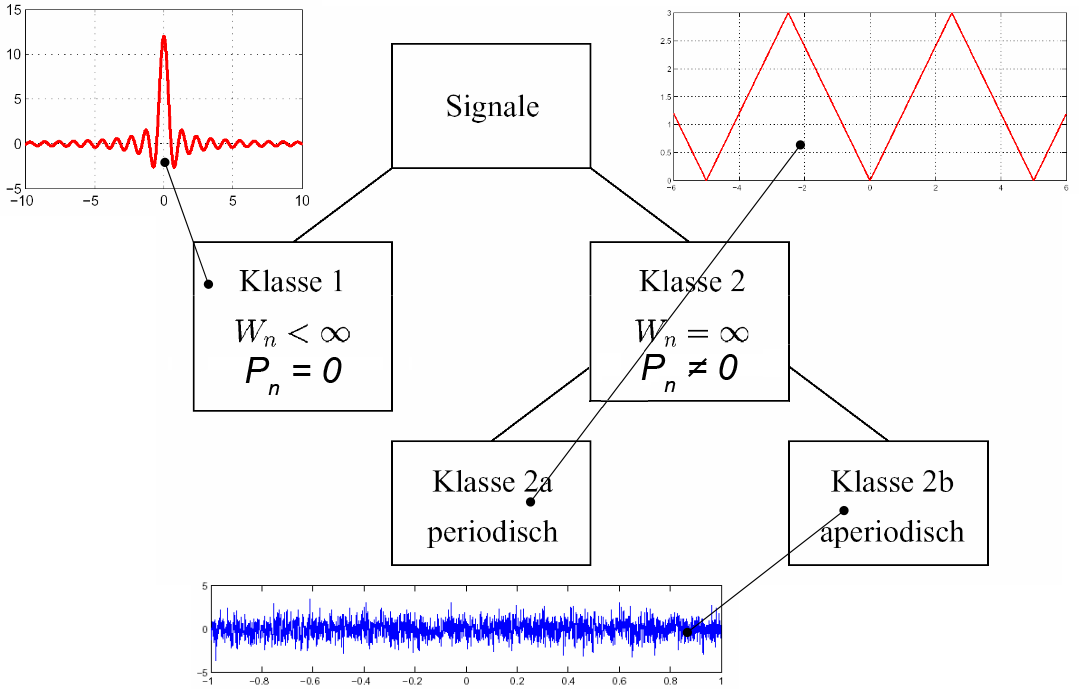
\includegraphics[width=12cm]{./bilder/signalklassen.png}}
	& \parbox{6cm}{
	Klasse 1: Energiesignal\\
	Klasse 2: Leistungssignal\\ \\
	Normierte Signalenergie 
	$$E_n = W_n = \lim\limits_{T\rightarrow\infty}\int\limits_{-T/2}^{T/2}
	|f(t)|^2dt$$
	$$E_n = \frac{1}{2 \pi} \int\limits_{-\infty}^{\infty} |F(j \omega)|^2 d \omega$$ 
	
	Normierte Signalleistung
	$$P_n = \lim\limits_{T\rightarrow\infty}\frac{1}{T}\int\limits_{-T/2}^{T/2}
	|f(t)|^2dt$$ 
	$$P_n = \frac{1}{2 \pi} \int\limits_{-\infty}^{\infty} \left( \lim\limits_{T
	\rightarrow \infty} \frac{|F(j \omega)|^2}{T} \right) d \omega$$ }
\end{tabular}

\subsection{Mittelwerte \skript{5}}
\begin{tabular}{p{5cm}p{5.5cm}p{7.5cm}}
Arithmetischer Mittelwert, Gleichwert, Linearer MW &
	\fbox{$X_0 = \overline{X} = X_m = \frac {1} {T} \int\limits_{t_0}^{t_0+T} x(t)dt$} &
	\begin{minipage}{7.5cm}
    		Ist die Fläche unter der Zeitfunktion über eine Periode.
    \end{minipage} \\
Quadratischer MW, Leistung &
	\fbox{$X^2 = \frac {1} {T} \int\limits_{t_0}^{t_0+T} x^2(t)dt$} & 
	$X^n = \frac {1} {T} \int\limits_{t_0}^{t_0+T} x^n(t)dt$ (MW $n$. Ordnung) \\
Effektivwert &
	\fbox{$X = X_{\text{eff}}= \sqrt{X^2} = \sqrt{\frac{1}{T} \int\limits ^{t_0+T} _{t_0}{x^2(t)dt}}$}
	& \\ Gleichrichtwert &
	\fbox{$X_{|m|} = \bar{|X|} = \frac{1}{T} \int\limits_{t_0}^{t_0+T}{|x(t)| dt}$} &
	\begin{minipage}{7.5cm}
    	Arithm. Mittelwert der Zweiweggleichrichterschaltung
    \end{minipage} \\

	Varianz, Standardabweichung
	& \fbox{$\text{Var}(x)=\sigma^2= \frac {1} {T} \int\limits_{-T/2}^{T/2}
	(x(t)-X_0)^2dt = X^2-X_0^2$}
	& $\qquad \qquad \qquad$ Mittl. Fehler im Quadrat
\end{tabular}
\\ \\	


\newpage
\subsection{Funktionen}
\begin{tabular}{ll}
\textbf{Autokorrelationsfunktion (AKF)}
	& ``Wie weit wird die Zukunft von der Vergangenheit geprägt?'' \\
\parbox{6cm}{
	\skript{8}\\
	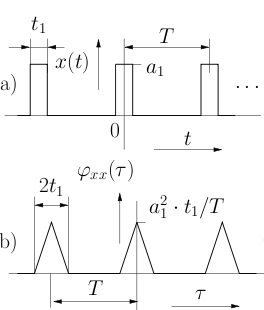
\includegraphics[width=4cm]{./bilder/akf1.png}\\
	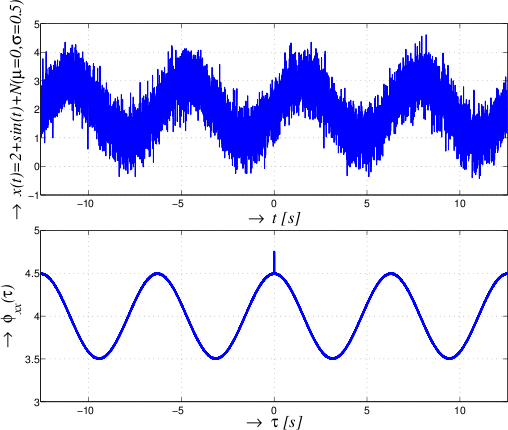
\includegraphics[width=4cm]{./bilder/akf2.png}
	} 
	& \parbox{12cm}{
	Für \textbf{Energiesignale} (Klasse 1):
	$$\varphi_{xx}(\tau) = \lim_{T\rightarrow\infty}\int\limits_{-T/2}^{T/2}
	x(t)x(t-\tau)dt=
	\lim_{T\rightarrow\infty}\int\limits_{-T/2}^{T/2} x(t+\tau)x(t)dt =
	\varphi_{xx}(-\tau)$$
	
	Für \textbf{periodische Leistungssignale} (Klasse 2a):
	$$\varphi_{xx}(\tau) = \frac {1} {T}
	\int\limits_{-T/2}^{T/2} x(t)x(t-\tau)dt 
	= \frac {1} {T} \int\limits_{-T/2}^{T/2} x(t+\tau)x(t)dt =
	\varphi_{xx}(-\tau)$$
	
	Für \textbf{nichtperiodische, stochastische Leistungssignale} (Klasse 2b):
	$$\varphi_{xx}(\tau) = \lim_{T\rightarrow\infty} \frac {1} {T}
	\int\limits_{-T/2}^{T/2} x(t)x(t-\tau)dt=\lim_{T\rightarrow\infty}\frac {1}
	{T} \int\limits_{-T/2}^{T/2} x(t+\tau)x(t)dt = \varphi_{xx}(-\tau)$$
	
	\textbf{Eigenschaften}
	\begin{itemize}
     \item $\varphi_{xx}(0) = X^2$ (Hat immer Diracstoss bei $\tau = 0$)
     \item $\varphi_{xx}(\tau)=\varphi_{xx}(\tau\pm mT)$, d.h. die
     AKF\index{Autokorrelationsfunktion} ist periodisch mit der gleichen Periode
     $T$ wie das Signal $x(t)$.
	\item $\varphi_{xx}(\tau)=\varphi_{xx}(-\tau)$: d.h. die AKF ist eine {\bf
	gerade Funktion}
	\item $\varphi_{xx}(0)\geq|\varphi_{xx}(\tau)|\quad$
	\item $\varphi_{xx}(\tau)\geq (X_0)^2-\sigma^2\quad$
   \end{itemize}
   
   $x(t) = a_k \cos(\omega t + \varphi) \Rightarrow \varphi_{xx}(t) =
   \frac{a_k^2}{2} \cos(\omega t)$\\
   $x(t) = b_k \sin(\omega t + \varphi) \Rightarrow \varphi_{xx}(t) =
   \frac{b_k^2}{2} \cos(\omega t)$\\ } \\
\hline & \\
\textbf{Kreuzkorrelationsfunktion (KKF)}
	& ``Wie ähnlich sind sich zwei Signale?'' \matlab{xcorr}\\
\parbox{6cm}{
 	\skript{11} \\
	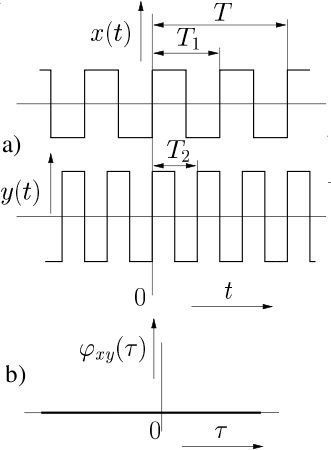
\includegraphics[width=4cm]{./bilder/kkf.png}
	}
	& \parbox{12cm}{
	Für \textbf{Energiesignale} (Klasse 1):
	$$\varphi_{xy}(\tau) = \lim_{T\rightarrow\infty}\int\limits_{-T/2}^{T/2}
	x(t)y(t-\tau)dt =\int\limits_{-T/2}^{T/2} x(t+\tau)y(t)dt$$ 

	Für \textbf{periodische Leistungssignale} (Klasse 2a):
	$$\varphi_{xy}(\tau) = \frac {1} {T} \int\limits_{-T/2}^{T/2}  x(t)y(t-\tau)dt
	= \frac {1} {T} \int\limits_{-T/2}^{T/2}  x(t+\tau)y(t)dt$$ 
		
	Für \textbf{nichtperiodische, stochastische Leistungssignale} (Klasse 2b):
	$$\varphi_{xy}(\tau) = \lim_{T\rightarrow\infty} \frac {1} {T}
	\int\limits_{-T/2}^{T/2}x(t)y(t-\tau)dt = \lim_{T\rightarrow\infty}\frac {1}
	{T} \int\limits_{-T/2}^{T/2} x(t+\tau)y(t)dt$$  
	
	Bei Signalen mit verschiedenen Frequenzen ist $\varphi_{xy}$ immer $0$!\\
	} \\
\end{tabular}

\newpage
\begin{tabular}{ll}
\textbf{Sprungfunktion \skript{16}}
	& Einschaltfunktion, Einheitssprung, Heaviside-Function \matlab{heaviside} \\
\parbox{6cm}{
	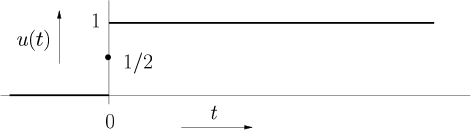
\includegraphics[width=5.5cm]{./bilder/sprungfunktion.png}
	}
	& \parbox{12cm}{
	$$u(t) = 1(t) = 
  \begin{cases}
    0 & \mbox{f"ur } t < 0,\\
    \frac{1}{2} & \mbox{f"ur } t = 0,\\
    1 & \mbox{f"ur } t > 0.\\
  \end{cases}$$	
	$$\mathcal{L:}\quad u(t) \FT \frac1s$$
	} \\

\hline & \\
\textbf{Signumfunktion \skript{16}}
	& Vorzeichenfunktion \matlab{sign} \\
\parbox{6cm}{
	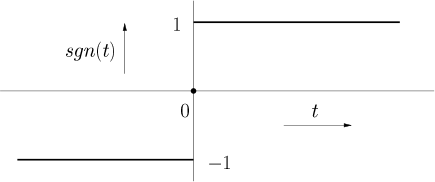
\includegraphics[width=5.5cm]{./bilder/sign.png}
	}
	
	& \parbox{12cm}{
	$$\sgn(t) =
  \begin{cases}
    -1 & \mbox{f"ur } t < 0,\\
    0 & \mbox{f"ur } t = 0,\\
    1 & \mbox{f"ur } t > 0.\\
  \end{cases}$$
	$$\mathcal{F:}\quad \sgn(t) \FT \frac{-2j}{\omega}$$
	\\
	} \\
\hline & \\

\textbf{Rampenfunktion \skript{17}}
	& \matlab{ramp} \\
\parbox{6cm}{
	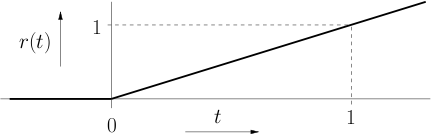
\includegraphics[width=5.5cm]{./bilder/ramp.png}
	}
	& \parbox{12cm}{
	$$r(t) = t u(t) =
  \begin{cases}
    0 & \mbox{f"ur } t \leq 0\\
    t & \mbox{f"ur } t > 0\\
  \end{cases}$$
	$$\mathcal{L:}\quad r(t) \FT \frac{1}{s^2}$$
	\\
	} \\
\hline & \\

\textbf{Rechteckimpuls \skript{17}}
	&  \\
\parbox{6cm}{
	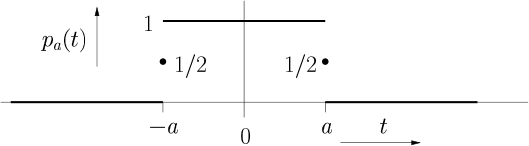
\includegraphics[width=5.5cm]{./bilder/rechteckimpuls.png}
	}
	& \parbox{12cm}{
	$$p_a(t) = u(t+a) -u(t-a) = 
  \begin{cases}
    1 & \mbox{f"ur } |t| < a\\
    \frac{1}{2} & \mbox{f"ur } |t| = a\\
    0 & \mbox{f"ur } |t| > a\\
  \end{cases}$$
	$$\mathcal{F:}\quad p_a(t) \FT 2a \sinc(a \omega) = \frac{2}{\omega} \sin(a \omega)$$
	\\
	} \\
\hline & \\

\textbf{Dreieckimpuls \skript{18}}
	&  \\
\parbox{6cm}{
	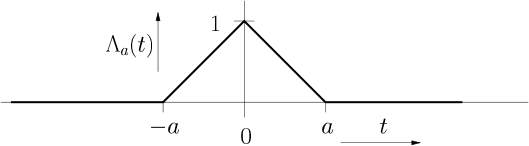
\includegraphics[width=5.5cm]{./bilder/dreieckimpuls.png}
	}
	& \parbox{12cm}{
	$$\Lambda_a(t) =
  \begin{cases}
    1 - \frac{|t|}{a}& \mbox{f"ur } |t| < a\\
    0 & \mbox{f"ur } |t| \geq a\\
  \end{cases}$$
	$$\mathcal{F:}\quad \Lambda_a(t) \FT
	a\left(\frac{\sin(\frac{a\omega}{2})}{\frac{a\omega}{2}}\right)^2 = a \sinc^2\left(\frac{a\omega}{2}\right)$$ \\
	} \\
\hline & \\

\textbf{Sincfunktion \skript{18}}
	& \matlab{sinc}  \\
\parbox{6cm}{
	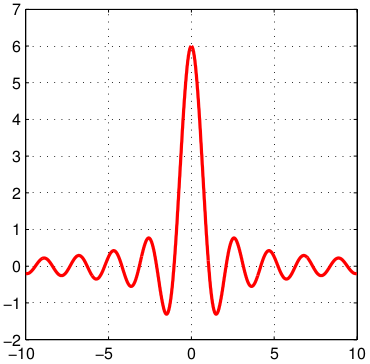
\includegraphics[width=5.5cm]{./bilder/sinc.png}
	}
	& \parbox{12cm}{
	$$ \sinc_{\alpha}(t) = \frac{\sin(\alpha t)}{t} \qquad 
	\sinc(\alpha t) = \frac{\sin(\alpha t)}{\alpha t}$$
	
	$$\mathcal{F:}\quad  \sinc_{\alpha}(t) = \frac{\sin(\alpha t)}{t} \FT
	\pi p_{\alpha}(\omega)$$
	$$\mathcal{F:}\quad  \sinc(\alpha t) = \frac{\sin(\alpha t)}{\alpha t} \FT
	\frac{\pi}{\alpha} p_{\alpha}(\omega)$$ } \\
\end{tabular}

\newpage
\begin{tabular}{ll}
\textbf{Impulsfunktion \skript{19}}
	& Diracimpuls, Diracstoss, Deltaimpuls \matlab{dirac} \\
\parbox{5cm}{
	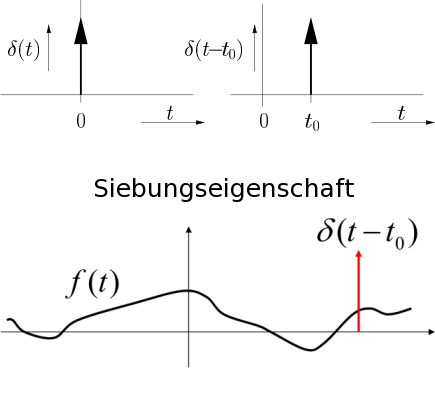
\includegraphics[width=5cm]{./bilder/dirac.png}
	}
	& \parbox{13cm}{
	$$\delta(t) =
  \begin{cases}
    \infty & \mbox{f"ur } t = 0\\
    0 & \mbox{sonst}\\
  \end{cases}$$
	\begin{tabular}{|r|c|l|}\hline
	 1. & $\delta(at) = \frac{1}{|a|}\delta(t)$ & Skalierung\index{Skalierung}\\ \hline
	 2. & $\delta(\frac{t-t_0}{a}) = |a|\cdot\delta(t-t_0)$ & Skalierung und Verschiebung  \\ \hline
	 3. & $\delta(-t+t_0) = \delta(t-t_0)$ & symmetrisch\\ \hline
	 4. & $\delta(-t) = \delta(t)$ & $\delta(t)=\mbox{ gerade Funktion}$ \\ \hline
	 \textbf{5.} & $\int\limits_{-\infty}^{\infty}\delta(t-t_0)f(t)dt = f(t_0)$ & \textbf{Siebungseigenschaft}\\ \hline
	 6. & $\delta(t-t_0)f(t) = f(t_0)\delta(t-t_0)$ &  Abtastung\index{Abtastung}\\ \hline
	 \textbf{7.} & $\int\limits_{-\infty}^{\infty}A\cdot\delta(t)dt = A$ & \textbf{Spezialfall der Siebungseigenschaft} \\ \hline
	 8. & $\delta(t-t_0)\ast f(t) = f(t-t_0)$ & Faltung\\ \hline
	 9. & $\delta(t-t_1)\ast\delta(t-t_2) = \delta(t-t_1-t_2)$ & Faltung\index{Faltung}\\ \hline
	10. & $\delta(t)=\frac{\partial u(t)}{\partial t}$ & Ableitung des Einheitssprungs\index{Ableitung}\\ \hline
	11. & $\delta(t)=\lim\limits_{\omega\rightarrow \infty}\frac{\sin(\omega
	t)}{\pi t}$ & Definition\\ \hline 
	12. & $\mathcal{L}, \mathcal{F}:\quad \delta(t) \FT 1$ 
		& Frequenzbereich \\ \hline
	\end{tabular}\\
	\vspace{.1cm}\\
	}
\end{tabular}


\begin{tabular}{ll}
\hline & \\
\textbf{Rauschen \skript{22}}
	& \matlab{randn} \\
\parbox{7cm}{
	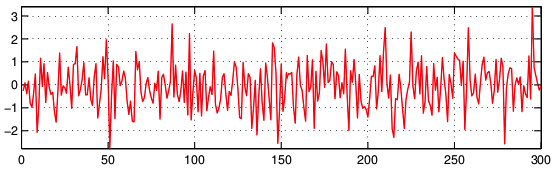
\includegraphics[width=7cm]{./bilder/rauschen.png}
	}
	& \parbox{11cm}{
	Ist die Intensit"at der
	Rauschspannung "uber viele Frequenzdekaden
	gleich verteilt, so spricht man von weissem Rauschen. \\
	Signal to Noise Ratio: $\text{SNR} =
	\frac{\text{Signalleistung}}{\text{Rauschleistung}}$ (rauschfrei $ \rightarrow
	\infty$) \\ \\ Effektive Rauschspannung / -leistung
	$$U_r = \sqrt { 4 \cdot k \cdot T \cdot \Delta f \cdot R}$$
	$$P_r = k \cdot T \cdot \Delta f$$
	} \\
\hline & \\
\end{tabular}

\subsection{Amplitudenanalyse \skript{24}}
\begin{tabular}{ll}
	& ``Zeit während sich Signal in bestimmtem Amplitudenintervall aufhält'' \\
\parbox{7cm}{
	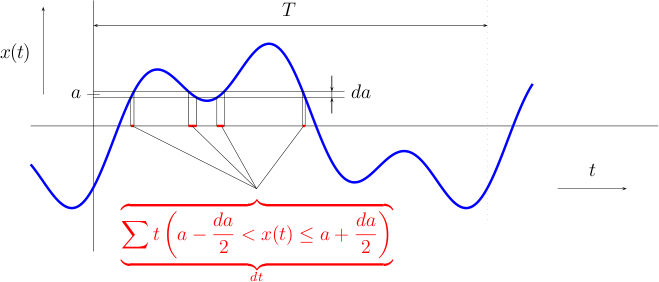
\includegraphics[width=7cm]{./bilder/amplitudenanalyse.png}
	}
	& \begin{minipage}[]{11cm}
			$$p(a) = \lim_{da\rightarrow 0}\frac{\underbrace{\sum t\left(
			a-\frac{da}{2}<x(t)\leq a+\frac{da}{2}\right)}_{dt}}{T\cdot da} = \frac{1}{T}\cdot
			\frac{1}{\partial a/ \partial t}$$
			$$\int p(a) da = 1$$
			
			\begin{tabular}{ll}
            Linearer Mittelwert 
            	& \fbox{$X_0  = \int\limits_{-\infty}^{\infty}a\cdot p(a)da$} \\ \\ 
            Mittelwert $n$. Ordnung 
            	& \fbox{$X^n = \int\limits_{-\infty}^{\infty}a^n\cdot p(a)da$} \\ \\
            \end{tabular}
      \end{minipage} \\
\end{tabular}
\newpage
\begin{center}
\textbf{Zusammenstellung verschiedener Verteilungen \skript{26}} \\
\begin{tabular}{|c|c|c|c|}\hline
Verteilung & gleichverteilt & gaussf"ormig & sinusf"ormig \\ \hline\hline
 & 
	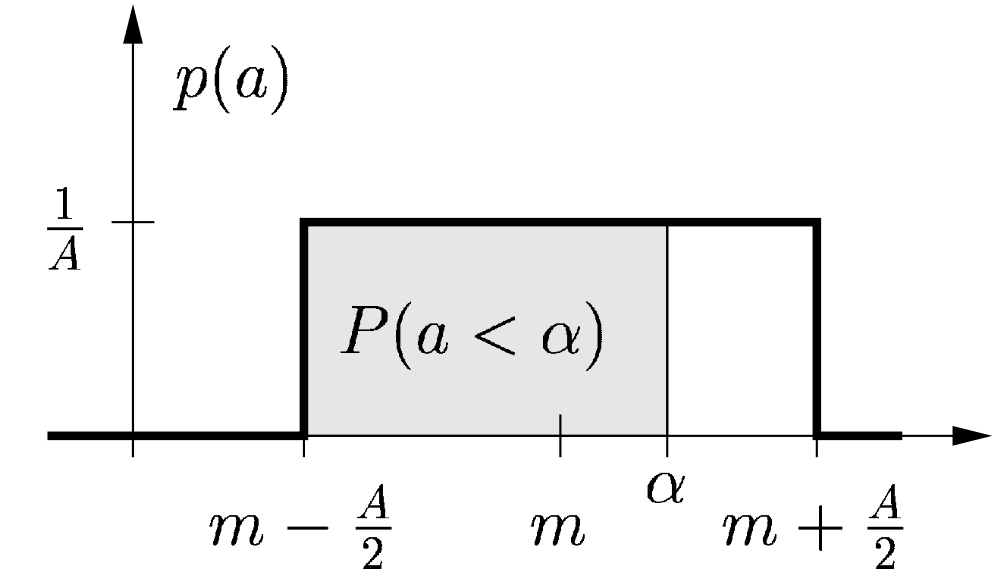
\includegraphics[width=4.3cm]{./bilder/verteilungen-gleichvert.png}
 &
	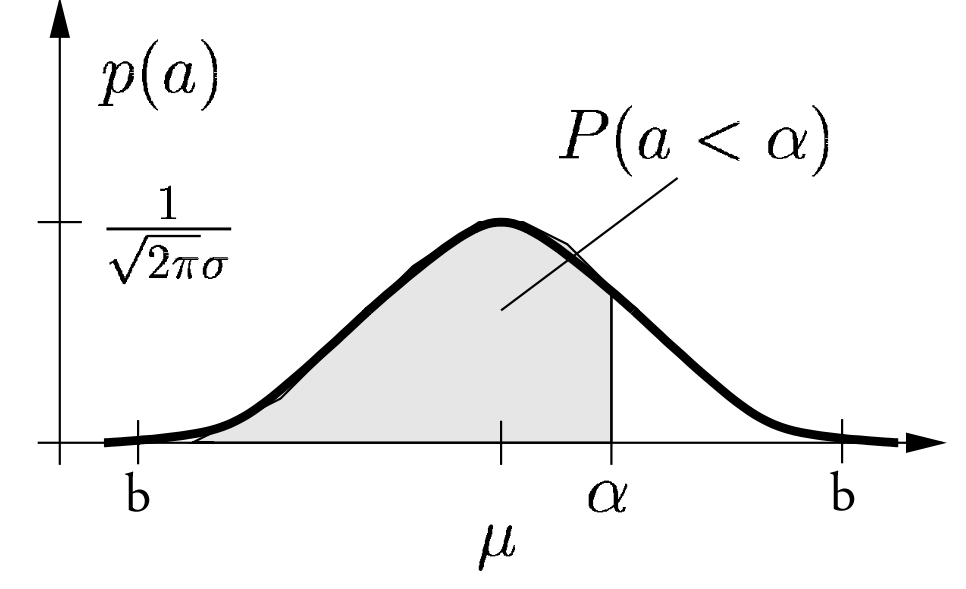
\includegraphics[width=4.3cm]{./bilder/verteilungen-gauss.png}
 &
	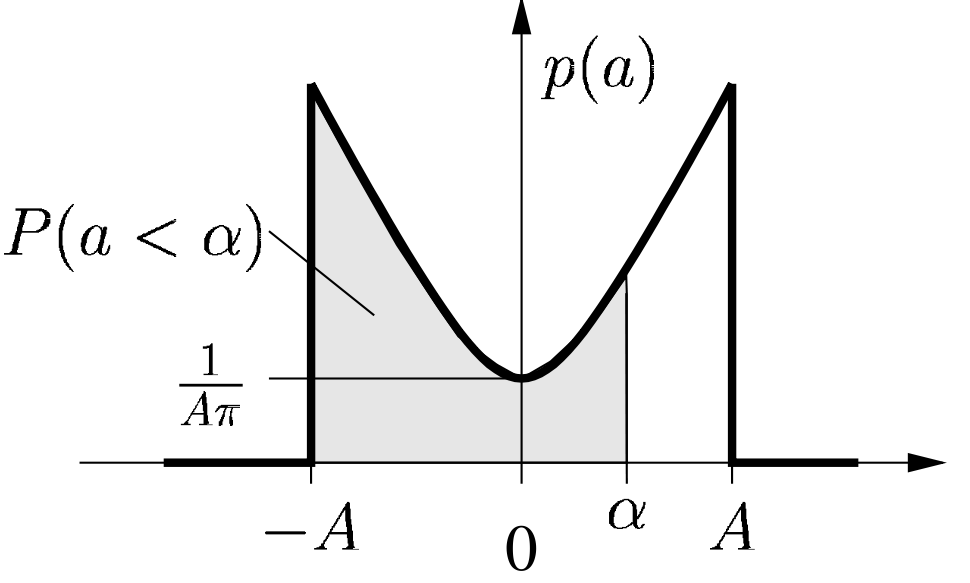
\includegraphics[width=4.3cm]{./bilder/verteilungen-sinus.png}\\ \hline 
Amplitudendichte & & & \\ $p(a)=$ & $\begin{cases} \frac{1}{A}&|a-m|\leq
\frac{A}{2},\\ 0&|a-m|>\frac{A}{2}.\\ \end{cases}$ &
$\displaystyle\frac{1}{\sqrt{2\pi}\sigma}e^{\displaystyle\frac{-(a-\mu)^2}{2\sigma^2}}$ & $\begin{cases} \frac{1}{\pi\sqrt{A^2-a^2}}&|a|\leq A,\\ 0&|a|>A.\\ \end{cases}$\\ \hline  
 Wahrscheinlichkeit,& & & \\ 
dass die Amplitude $a$ & & & \\  
kleiner gleich $\alpha$ ist& & & \\ 
$P(a\!\leq\!\alpha)\!=\!\!\int\limits_{-\infty}^{\alpha}\!p(a)da=$ &
$\begin{cases}0&\alpha<m-\frac{A}{2},\\ \frac{\alpha-(m-\frac{A}{2})}{A}&
|\alpha-m|\leq\frac{A}{2} \\1&\alpha\geq m+\frac{A}{2}. \end{cases}$  &
$Q\left(\frac{\displaystyle\mu-\alpha}{\displaystyle\sigma}\right)$ &
$\begin{cases}0&\alpha\!\leq\!-A,\\
\frac{1}{\pi}\left(\frac{\pi}{2}\!+\!\sin^{-1}\!\left(\frac{a}{A}\right)\right)&
|\alpha|\!<\!A,\\1&\alpha\geq A. \end{cases}$ \\ \hline      
 & & & \\ 
Mittelwert $X_0 =$& $m$ & $\mu$ & 0 \\ 
& & & \\ \hline
& & & \\
Varianz $\operatorname{Var}(x) = $& $\dfrac{A^2}{12}$
& $\sigma^2$ & $\dfrac{A^2}{2}$ \\ & & & \\ \hline
& & & \\
Leistung $X^2 =$& $m^2+\dfrac{A^2}{12}$ &
$\mu^2+\sigma^2$ & $\dfrac{A^2}{2}$ \\ 
& & & \\ \hline
\end{tabular}
\end{center}

\begin{tabular}{ll}
\textbf{Faltung \skript{28}}
	& Convolution, ``Addition zweier unabhängiger ergodischer Prozesse $n_i$'' \matlab{conv} \\
\parbox{5cm}{
	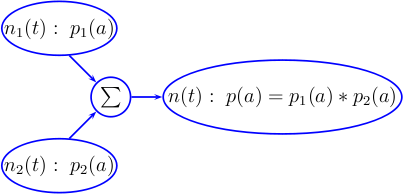
\includegraphics[width=5cm]{./bilder/faltung.png}
	\\}
	& \parbox{13cm}{
	$p(a) =
	\int\limits_{-\infty}^{\infty}p_1(\xi)\cdot p_2(a-\xi) d\xi = p_1(a)
	\ast p_2(a) =  p_2(a) \ast p_1(a) = \int\limits_{-\infty}^{\infty}p_2(\xi)\cdot 
  	p_1(a-\xi) d\xi$ \\
  	Die Breite des Faltungsproduktes entspricht der Summe der Breite der
  	einzelnen Faktoren.\\ \\
  	Faltung im Zeitbereich $\rightarrow$ Multiplikation im Frequenzbereich 
  	$$f(t) * g(t) \FT F(s) G(s)$$
  	Faltung im Frequenzbereich $\rightarrow$ Multiplikation im Zeitbereich
  	$$F(s) * G(s) \IFT \frac{1}{2 \pi} f(t) g(t)$$ } \\
\end{tabular}

\begin{tabular}{ll}
\hline & \\
\textbf{Q-Funktion \skript{35}}
	& ``Wahrscheinlichkeit eines Fehlers'' \matlab{erf, erfc} \\
\parbox{6cm}{
	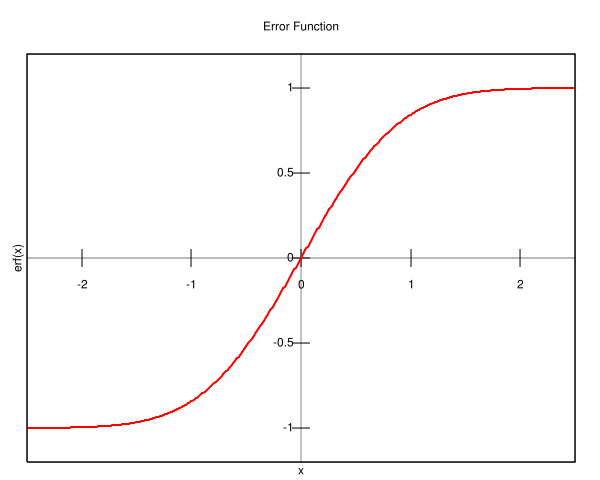
\includegraphics[width=5cm]{./bilder/q-funktion.png}
	}
	& \parbox{12cm}{
		Wenn die Resultate einer Messserie mit einer Normalverteilung mit Varianz
		$\sigma$ und Erwartungswert $0$ auftreten, dann ist
		$\operatorname{erf}\,\left(\,\frac{a}{\sigma \sqrt{2}}\,\right)$ die
		Wahrscheinlichkeit, dass ein einzelner Messwert zwischen $-a$ und $a$ liegt. 
		\\
		Tabelle \skript{44}\\
		$$Q(\xi)=\frac{1}{\sqrt{2\pi}}\int\limits_{\xi}^{\infty}
		e^{-\frac{y^2}{2}}dy$$
		$$Q(\xi) = \frac12 \operatorname{erfc}\left(\frac{\xi}{\sqrt2}\right)
		= \frac12 \left(1 - \operatorname{erf}\left( \frac{\xi}{\sqrt2}\right) \right)
		$$ }
\end{tabular}

\newpage
\section{Systeme \skript{95}}
\subsection{Begriffe}
\begin{tabular}{|p{5cm}|p{5cm}|p{7.5cm}|}
\hline & & \\
\textit{Bezeichnung}
	& \textit{Beschreibung}
	& \textit{Bedingung, Erkennung} \\
\hline \hline & & \\
Wirkungsfreiheit \skript{95}
	& Eingang des System hochohmig 
	& Kaskadierte Systeme durch Einheitsverstärker verbunden\\
\hline & & \\
Statische bzw. dynamische Systeme \skript{96}
	& Ohne bzw. mit Gedächtnis
	& Statisch: $u_2(t)$ nur vom Eingangssignal $u_1(t)$ bei $t$ abhängig \\
	& & Dynamisch: $\int dt; \; \frac{d}{dt}; \; f(t \pm t_0) $\\
\hline & & \\
Kausale bzw. akausale Systeme \skript{99}
	& Keine zukünftigen Werte bzw. nicht in ``Echtzeit''
	& \parbox{7cm}{Kausal: $f(t - t_0); \int^t f(\tau) d \tau \quad (t_0 > 0) \quad$ \\ Statische
	Systeme sind immer kausal. \\ \\ Akausal: $f(-t); \; f(t + t_0); \; \int^{t+t_0}
	f(\tau) d \tau$} \\
	\hline & & \\ Zeitinvariante bzw. zeitvariante Systeme  \skript{104} & Von der Zeit (un-) abhängig
	& \parbox{7cm}{Zeitvariant: $\cos(t) x(t); t^{\alpha} x(t) \quad \text{(} \alpha \neq 0 \text{)} $
	\\ \\ Zeitinvariant: $S(x(t-t_0)=S(x)\cdot x(t-t_0)$} \\
\hline & & \\
Lineare bzw. nichtlineare Systeme \skript{105}
	&
	& \parbox{7cm}{Nichtlinear: $f^{\alpha}(t); \; \alpha + f(t) $ \\ Kennlinie nicht durch
	Ursprung.\\ \\ Linear: $S(x1+x2)=S(x1)+S(x2)$ \\ $S(c\cdot x)=c\cdot S(x)$} \\
\hline 
\end{tabular}

\subsection{Übertragungsfunktion von LTI-Systemen \skript{108}}
\begin{tabular}{ll}
\parbox{13cm}{
	$$h(t) \FT H(s)$$
	$$s_2(t) = h(t) * s_1(t) \FT S_2(s) = H(s) S_1(s)$$}
	& \parbox{5cm}{
		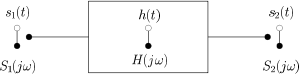
\includegraphics[width=5cm]{./bilder/utf-theorie.png}}\\
\multicolumn{2}{l}{Kaskadierung von wirkungsfreien Systemen:
$H_{total}(s) = H_1(s) H_2(s)$ bzw. bei $n$ gleichen Systemen:
$H_{total} = (H(s))^n$}
 \\ \\

\parbox{13cm}{
	\textbf{Beispiel}: Gesucht UTF $H(s) = \frac{Y(s)}{X(s)}$ \\
	$$H(s) = \frac{sL}{\frac{1}{sC} + sL + R} = \frac{s^2}{\frac{1}{LC} + s
	\frac{R}{L} + s^2}$$\\
	$$\Longrightarrow \text{Pole bei } s = -\frac{R}{2L} \pm j
	\sqrt{\frac{1}{LC} - \left(\frac{R}{2L}\right)^2} \quad ; \quad \text{Doppelte
	Nullstelle bei } s = 0$$
	Differentialgleichung:    $ \ddot{y}(t)+
	\frac{R}{L}\dot{y}(t)+\frac{1}{LC}y=\ddot{x}(t)$}
	
	
	& \parbox{5cm}{
		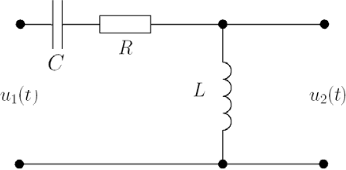
\includegraphics[width=5cm]{./bilder/utf-beispiel.png}} \\
		
\end{tabular}

\subsection{Berechnung des Amplituden- und Phasengangs aus der
Übertragungsfunktion}
$$H(j \omega) = \frac{Y(j \omega)}{X(j \omega)} = \underbrace{|H(j
\omega)|}_{Amplitudengang} e^{j\underbrace{\Theta(\omega)}_{Phasengang}} = 
\frac{|Y(j \omega)|}{|X(j \omega)|} e^{j (\arg(Y(j \omega)) - \arg(X(j
\omega)))} =
\frac{|Y(j \omega)|}{|X(j \omega)|} e^{j \left[\arctan \left(\frac{\Imag\{Y(j
\omega)\}}{\Real\{Y(j \omega)\}} \right) - \arctan \left(\frac{\Imag\{X(j
\omega)\}}{\Real\{X(j \omega)\}} \right)\right]}$$

\subsection{Zusammenhang zwischen Impuls- \& Einheitssprungantwort, Endwerte
\skript{109}}
$ \text{Einheitssprungantwort } g(t) \text{, Impulsantwort }h(t)$
$$h(t)= \frac{\partial g(t)}{\partial t}\quad\text{bzw.}\quad
g(t)=\int_{-\infty}^{t}h(\tau)d\tau \qquad;\qquad 
\lim\limits_{t \rightarrow \infty}  h(t)= \lim\limits_{s \rightarrow 0} s H(s)
\qquad;\qquad
\lim\limits_{t \rightarrow \infty}  g(t)= \lim\limits_{s \rightarrow 0} H(s)$$

\subsection{Phasen- \& Gruppenlaufzeit \skript{116}}
\definecolor{gruppe}{rgb}{1,.75,0} % 255,192,0
\definecolor{phase}{rgb}{1,0,0} % 255,0,0
Die \textcolor{phase}{Phasenlaufzeit}  ist nur für reine Sinussignale bestimmbar:
$\tau_P(\omega)=\frac{-\theta(\omega)}{\omega}$ \\
Die \textcolor{gruppe}{Gruppenlaufzeit} hingegen ist für sämtliche Signale möglich:
$\tau_G(\omega)=\frac{-\partial\theta(\omega)}{\partial\omega}$\\
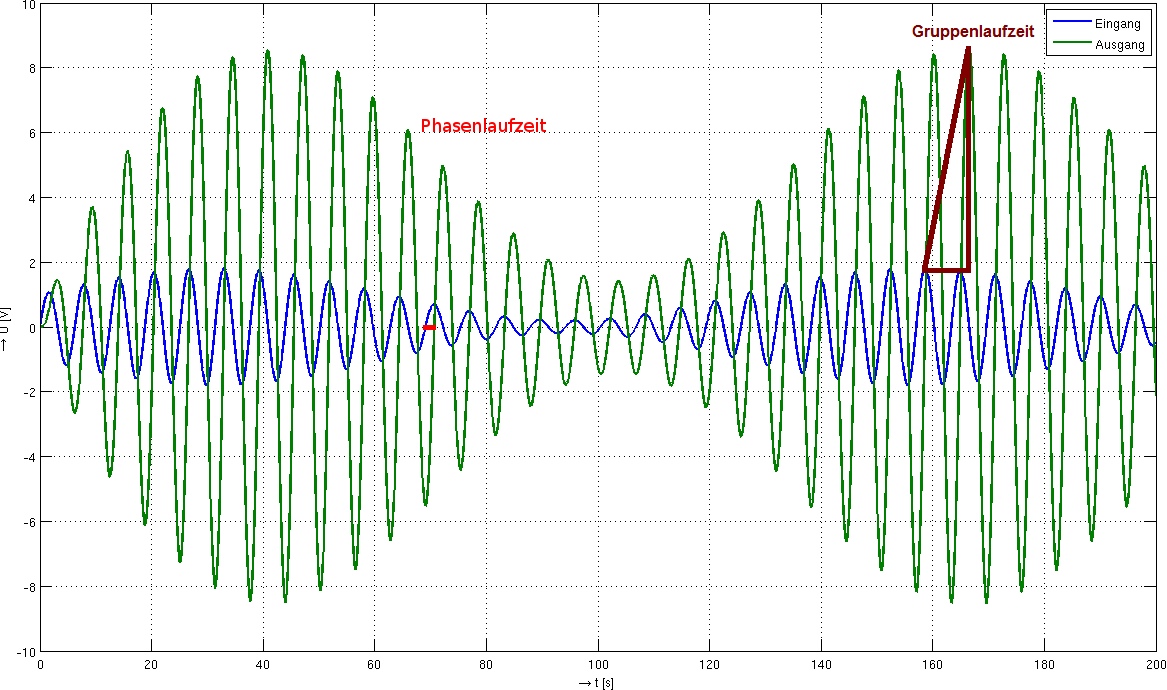
\includegraphics[width=18cm]{./bilder/laufzeit.png}\\
Eingangssignal $x(t)$ und Ausgangssignal $y(t)$ des Systems
$H(s)=\frac{1}{s^2+0.2s+1}$. Bemerkung: $y(t)$ ist gr"osser als $x(t)$.

\subsection{Stabilität von LTI-Systemen}
\subsubsection{Asymptotische Stabilität \skript{112}}
\begin{tabular}{ll}
Stabil: 
	& $\lim\limits_{t\rightarrow\infty} h(t) = 0$ 
	\qquad Pole \textbf{nur} in der
linken s-Halbebene.\\
Instabil: 
	& Mind. ein Pol in der rechten s-Halbebene oder mind. ein
\textbf{mehrfacher} Pol auf der $j$-Achse der s-Ebene. \\
Grenzstabil:
	& mindestens ein \textbf{einfacher Pol} auf der $j$-Achse
\end{tabular}

\subsubsection{Stabilität mit Hurwitz-Polynom \skript{113}}
Es wird jeweils das Polynom im \textbf{Nenner der Übertragungsfunktion} betrachtet:
$P(s) = a_n s^n + a_{n-1} s^{n-1} +\ldots +a_1s + a_0$ \\
\begin{tabular}{|l||l| l|}\hline
$N$   &   $P(s)$ ist ein Hurwitz-Polynom (stabil) &  $P(s)$ ist ein
modifiziertes Hurwitz-Polynom (grenzstabil) \\ \hline\hline
      1     &      gilt f"ur alle $P(s)$          &  $a_0=0$ \\ \hline
      2     &     gilt f"ur alle $P(s)$           &  $a_1=0$ \\ \hline
      3     &     $a_1a_2>a_0a_3$      &  $a_1a_2=a_0a_3$ \\ \hline
      4     &     $a_3(a_1a_2-a_0a_3)>a_1^2a_4$   &    $a_3(a_1a_2-a_0a_3)=a_1^2a_4$\\ \hline

      5    &     {\footnotesize $a_3a_4>a_2a_5$  und}   &     {\footnotesize $a_3a_4>a_2a_5$} \\
           &     {\footnotesize
           $(a_1a_2-a_0a_3)(a_3a_4-a_2a_5)>(a_1a_4-a_0a_5)^2$}   &  
           {\footnotesize $(a_1a_2-a_0a_3)(a_3a_4-a_2a_5)=(a_1a_4-a_0a_5)^2$} 
           \\ \hline   
\end{tabular}\\
\begin{itemize}
  \item Wenn \textbf{ein Koeffizient negativ} ist $(a_x < 0)$, dann ist das System
  \textbf{instabil}.
  \item Wenn \textbf{alle Koeffizienten negativ} sind, kann $-1$ ausgeklammert
  werden und in den Zähler verschoben werden\\ $\Rightarrow$ \textbf{System
  stabil} oder \textbf{grenzstabil} (siehe Punkt 3)
  \item Wenn \textbf{ein Koeffizient nicht vorhanden} ist $(a_x = 0)$, dann ist das System
  evtl. grenzstabil, d.h. es ist eine \textbf{Überprüfung mit modifiziertem Hurwitz-Polynom}
  nötig.
\end{itemize}

\subsection{Klirrfaktor \skript{122}}
Als Mass für nichtlineare Verzerrungen gilt der \textit{Klirrfaktor}. Betrachtet
wird jeweils der Effektivwert am Ausgang 
$$k = \sqrt{\frac{U_2^2 + U_3^2 + \ldots + U_n^2}{U_1^2 + U_2^2 + \ldots +
U_n^2}} \qquad 0 \leq k \leq 1$$ 
\begin{tabular}{ll}
Teilklirrfaktor (frequenzselektiv) 
	&$k_m =  \frac {U_m} {\sqrt{ U_1^2+ U_2^2 + \ldots + U_n^2} }$ \\
Klirrdämpfungsmass 
	& $a_k = 20 \log \left( \frac1k \right)$ $\qquad$ \\
Teilklirrdämpfungmass 
	& $a_k = 20 \log \left( \frac{1}{k_m} \right)$
\end{tabular}

\subsection{Total Harmonic Distortion (THD) \skript{122}}
$$\text{THD} = \sqrt{ \frac {U_2^2+ U_3^2 + \ldots + U_n^2} {U_1^2} } \qquad
\infty > \text{THD} \geq k \geq 0; \quad \text{Für kleine Verzerrungen: THD}
\approx k $$


\section{Zusammenstellung Signalformen}
\begin{table}[htdp]
\begin{center}
\begin{tabular}{|c|c|c|c|c|}
\hline
\textbf{Signal} & \textbf{$   X_0   $} & \textbf{$X^2$} & \textbf{var(X)} \\
\hline
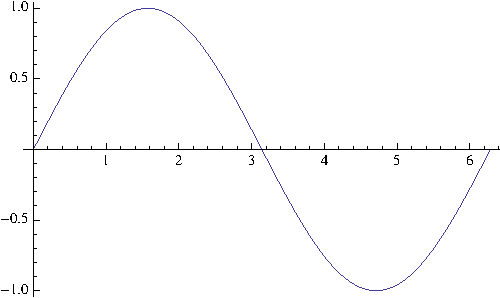
\includegraphics[height=2cm]{./bilder/Sinus.pdf} & $0$ & $\frac{A^2}{2}$ &
$\frac{A^2}{2}$ \\
\hline
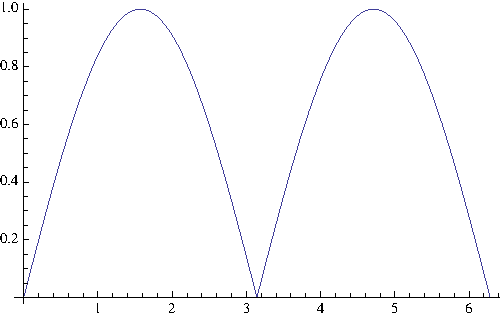
\includegraphics[height=2cm]{./bilder/absSinus.pdf}  & $\frac{2A}{\pi}$ &
$\frac{A^2}{2}$ & $\frac{A^2}{2}-\frac{4A^2}{\pi^2}$\\
\hline
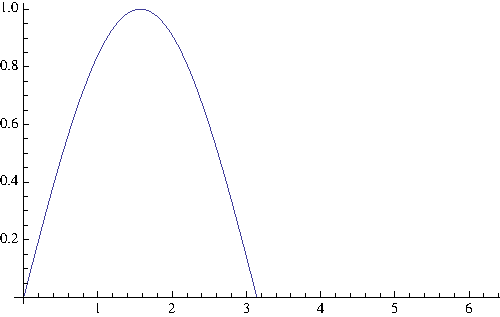
\includegraphics[height=2cm]{./bilder/halbSinus.pdf} & $\frac{A}{\pi}$ &
$\frac{A^2}{4}$ & $\frac{A^2}{4}-\frac{A^2}{\pi^2}$\\
\hline
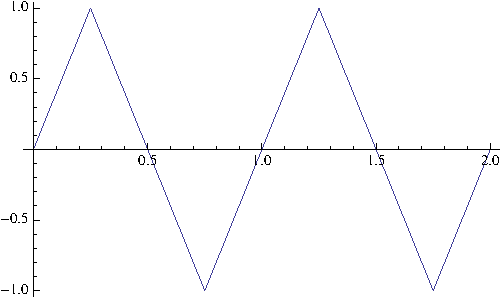
\includegraphics[height=2cm]{./bilder/triangular.pdf} & $0$ & $\frac{A^2}{3}$ &
$\frac{A^2}{3}$ \\
\hline
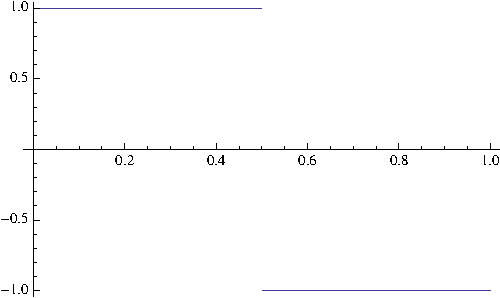
\includegraphics[height=2cm]{./bilder/square.pdf} & $0$ & $A^2$ & $A^2$ \\
\hline
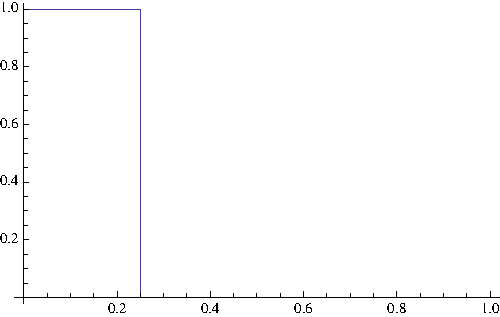
\includegraphics[height=2cm]{./bilder/pwm.pdf}  & $A\frac{t}{T}$ &
$A^2\frac{t}{T}$ & $\frac{A^2t}{T}-\frac{A^2t^2}{T^2}$ \\
\hline




\end{tabular}
\end{center}
\label{default}
\end{table}%

\end{document}
